\documentclass{article}

\usepackage{graphicx}
\usepackage{setspace}
\usepackage{listings}
\usepackage{color}

\definecolor{dkgreen}{rgb}{0,0.6,0}
\definecolor{gray}{rgb}{0.5,0.5,0.5}
\definecolor{mauve}{rgb}{0.58,0,0.82}

\lstset{frame=tb,
    language=VHDL,
    aboveskip=3mm,
    belowskip=3mm,
    showstringspaces=false,
    columns=flexible,
    basicstyle={\small\ttfamily},
    numbers=none,
    numberstyle=\tiny\color{gray},
    commentstyle\color{dkgreen},
    stringstyle=\color{mauve},
    breaklines=true,
    breakatwhitespace=true,
    tabsize=3
    }

\title{ECE 210 - Combinational Logic Design \\
    Lab 2}
\date{2018-10-24}
\author{David Lenfesty \\ lenfesty@ualberta.ca
    \and Radomir Wasowski \\ wasowski@ualberta.ca}

\setcounter{tocdepth}{2} % Show subsections

\begin{document}

    \pagenumbering{gobble}
    \maketitle
    \newpage

    \doublespacing
    \tableofcontents
    \newpage


    \singlespacing
    \pagenumbering{arabic}

    \section{Abstract}

    Various logic circuit designs can be combined together to create
    functional applications.

    Multiplexers and demultiplexers can be used to route specific
    incoming signals to a specified destination. In this lab a simulated
    digital signal from three different receivers was routed towards
    one of three "engineers".
    
    As well, logical elements can be used to design a simplistic access control system.
    In this lab such a circuit was designed and tested on an FPGA.

    \section{Introduction}

    The purpose of this lab was to design a simple Multiplexer and Demultiplexer circuit,
    as well as to design a circuit to control access to a lab.

    In order to validate the Multiplexer/Demultiplexer circuit,
    a useful circuit was designed using Xilinx Vivado software,
    and this circuit was simulated against the required inputs.

    In order to test the Lab Access Control circuit, the circuit was again designed
    using Xilinx Vivado, and simulated against required inputs.
    However, for this section, the design was also uploaded to a physical board
    where various inputs could be physically tested and validated.

    \section{Design Section}

    In order to design the following circuits, the Xilinx Vivado software
    was used to write VHDL that described the logic circuit.

    \paragraph{MUX / DEMUX Circuit}


    \begin{lstlisting}
entity lab2_part1 is
    Port ( clk : in STD_LOGIC;
           I  : in STD_LOGIC_VECTOR (2 downto 0);
           O  : out STD_LOGIC_VECTOR (2 downto 0);
           EI : out STD_LOGIC_VECTOR (2 downto 0);
           S  : in STD_LOGIC_VECTOR (1 downto 0);
           DS : in STD_LOGIC_VECTOR (1 downto 0) );
end lab2_part1;

architecture Behavioral of lab2_part1 is
    signal M   : STD_LOGIC := '0';
    signal SEL : STD_LOGIC_VECTOR (2 downto 0) := "000";
    
begin

    M <= ((not S(1) and not S(0)) and I(0)) or ((not S(1) and S(0)) and I(1)) or (( S(1) and not S(0) ) and I(2));
    
    SEL(0) <= (not DS(1) and not DS(0));
    SEL(1) <= (not DS(1) and DS(0));
    SEL(2) <= (DS(1) and not DS(0)); 
    
    O(0) <= M and SEL(0);
    O(1) <= M and SEL(1);
    O(2) <= M and SEL(2);
    
    EI(0) <= SEL(0);
    EI(1) <= SEL(1);
    EI(2) <= SEL(2);

end Behavioral;
    \end{lstlisting}

    \paragraph{Lab Access Control Circuit}

    \section{Procedure}
    We typed things

    \paragraph{Part 1}

    Simu

    \paragraph{Part 2}


    \section{Results}
    Lights flashed

    \begin{figure}[b!]
        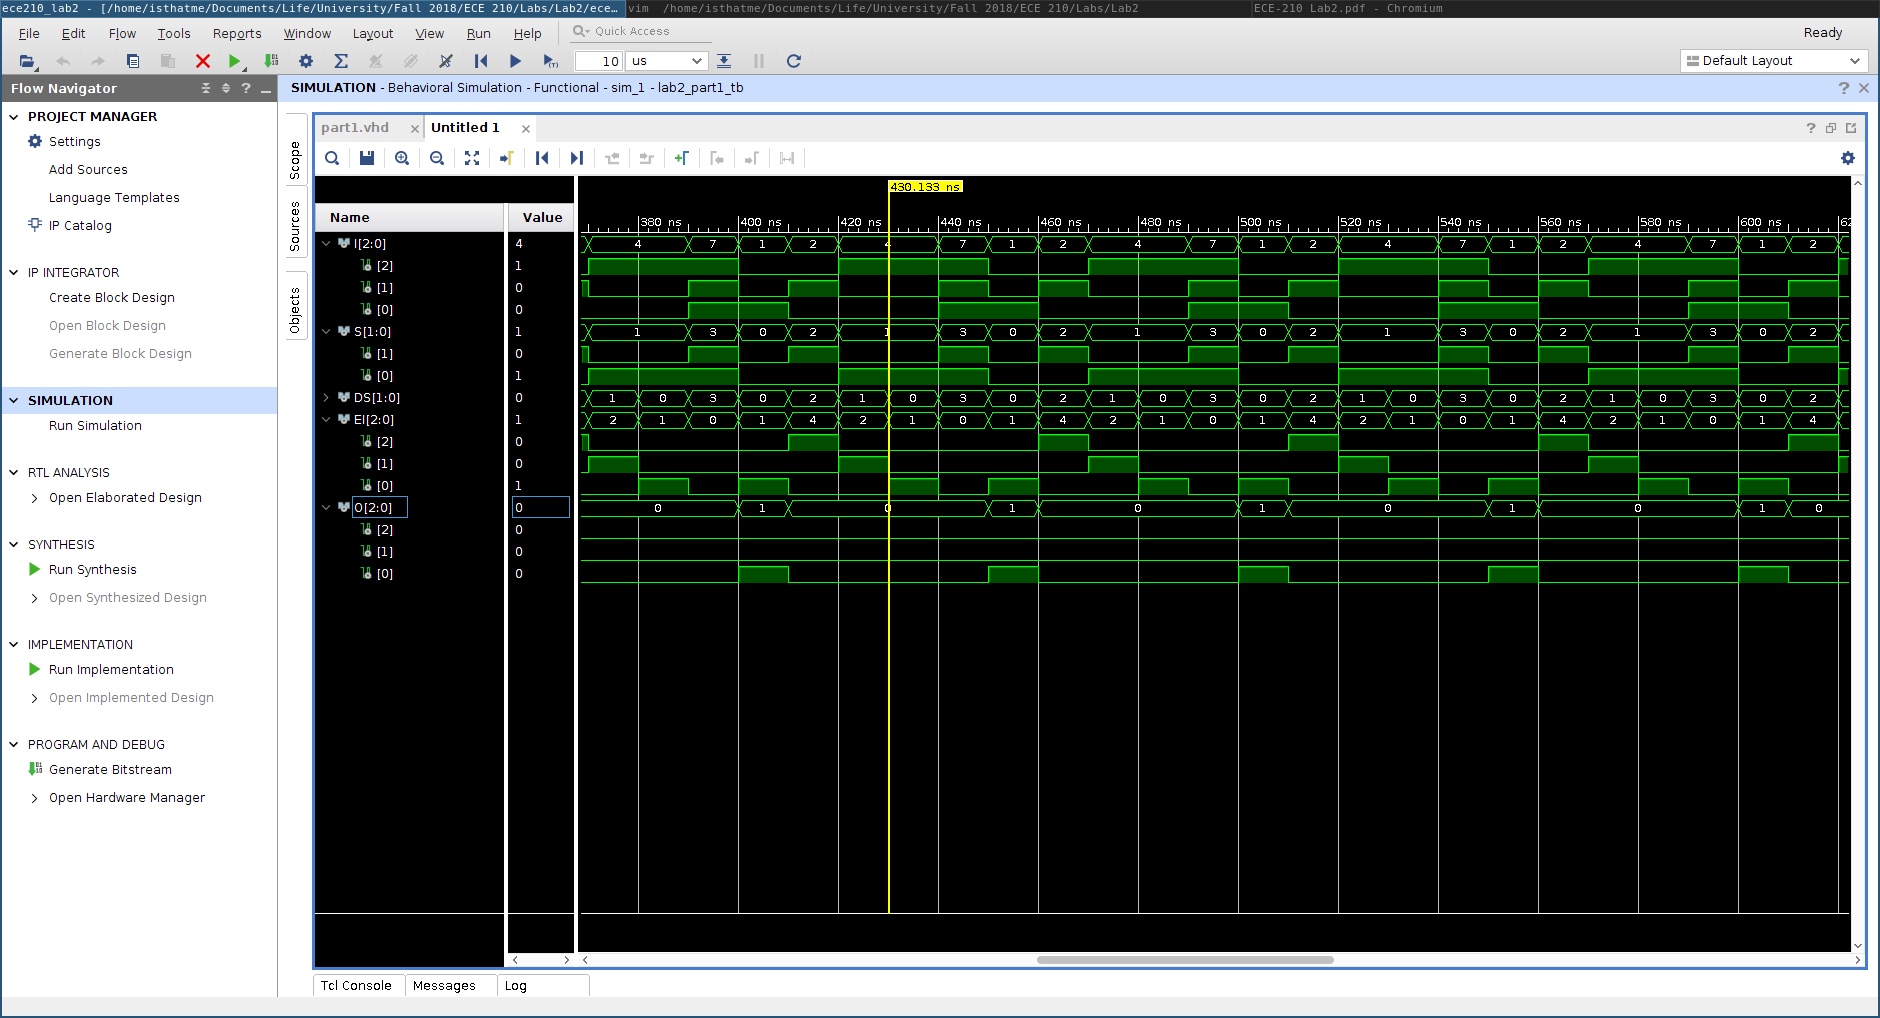
\includegraphics[width=\linewidth]{MUX_DEMUX.png}
        \caption{Part 1 Simulation.}
        \label{fig:part1_sim}
    \end{figure}

    \paragraph{Part 1}


    \paragraph{Part 2}


    \section{Discussion}
    Dogs are better than cats.
    End of discussion

    \section{Conclusion}
    Blinkies are cool.


\end{document}

